\documentclass[12pt,letterpaper]{exam}
\usepackage[lmargin=1in,rmargin=1in,tmargin=1in,bmargin=1in]{geometry}
\usepackage{../style/exams}

% -------------------
% Course & Exam Information
% -------------------
\newcommand{\course}{MAT 101: Exam 2}
\newcommand{\term}{Fall -- 2023}
\newcommand{\examdate}{11/08/2023}
\newcommand{\timelimit}{85 Minutes}

\setbool{hideans}{true} % Student: True; Instructor: False

% -------------------
% Content
% -------------------
\begin{document}

\examtitle
\instructions{Write your name on the appropriate line on the exam cover sheet. This exam contains \numpages\ pages (including this cover page) and \numquestions\ questions. Check that you have every page of the exam. Answer the questions in the spaces provided on the question sheets. Be sure to answer every part of each question and show all your work. If you run out of room for an answer, continue on the back of the page --- being sure to indicate the problem number.} 
\scores
\bottomline
\newpage

% ---------
% Questions
% ---------
\begin{questions}

% Question 
\newpage
\question[10] Consider the relation $f$ shown below. 
	\[
	\fbox{
	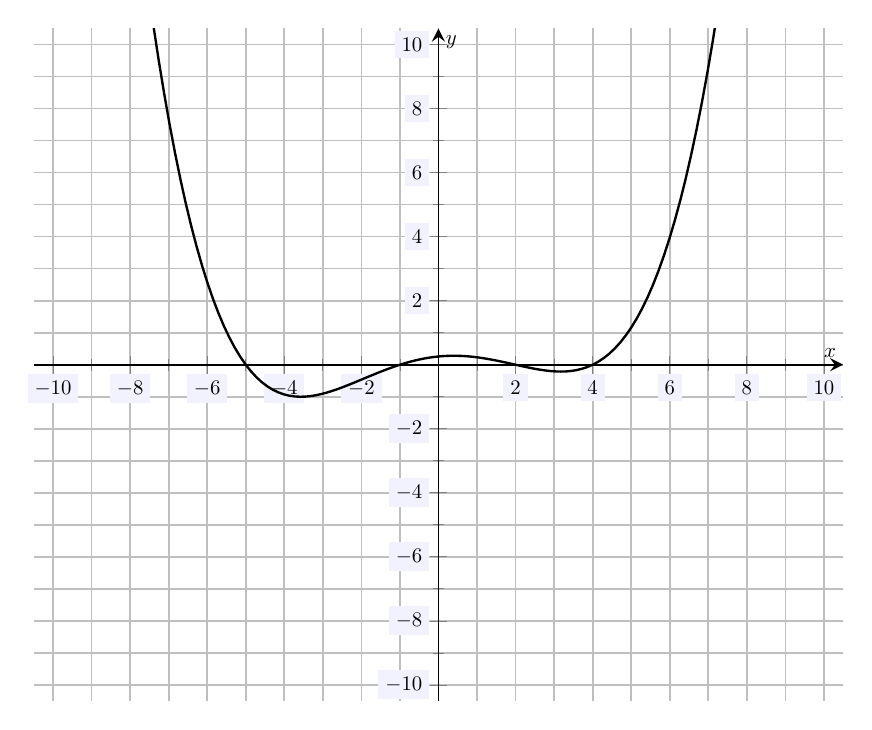
\begin{tikzpicture}[scale=1.5,every node/.style={scale=0.5}]
	\begin{axis}[
	grid=both,
	axis lines=middle,
	ticklabel style={fill=blue!5!white},
	xmin= -10.5, xmax=10.5,
	ymin= -10.5, ymax=10.5,
	xtick={-10,-8,-6,-4,-2,0,2,4,6,8,10},
	ytick={-10,-8,-6,-4,-2,0,2,4,6,8,10},
	minor tick = {-10,-9,...,10},
	xlabel=\(x\),ylabel=\(y\),
	]
	\addplot[line width= 0.02cm,samples=150,domain= -10.5:10.5] ({x},{1/155*(x - 4)*(x - 2)*(x + 1)*(x + 5)});
	\end{axis}
	\end{tikzpicture}
	}
	\] 

\begin{enumerate}[(a)]
\item Is the relation shown above a function of $x$? Explain. 
\item Assuming the relation is a function of $x$, does the relation above have an inverse that is a function of $y$? Explain.
\item Find $f(6)$.
\item Find the $x$-intercepts of $f(x)$.
\item Is there an $x$ such that $f(x)= 2$? Explain. 
\end{enumerate}



% Question 2
\newpage
\question[10] Consider invertible functions $f, g$, whose values at several specified $x$-values are given below. 
	\begin{table}[h]
	\centering
	\begin{tabular}{|c||c|c|c|c|c|} \hline
	$x$ & $-6$ & $2$ & $0$ & $5$ & $9$ \\ \hline
	$f$ & $1$ & $5$ & $2$ & $-6$ & $3$ \\ \hline
	$g$ & $0$ & $2$ & $7$ & $1$ & $6$ \\ \hline
	\end{tabular}
	\end{table}
Find the following:
	\begin{enumerate}[(a)]
	\item $(f + g)(9)$
	\item $(f \circ g)(0)$
	\item $\left( \frac{g}{f} \right)(2)$
	\item $y$-intercept of $f(x)$
	\item An $x$-intercept of $g(x)$
	\end{enumerate}



% Question 3
\newpage
\question[10] Let $f(x)= x^2 + 2x - 1$, $g(x)= 3x + 8$, and $c$ be a constant. Showing all your work and simplifying as much as possible, compute the following:
	\begin{enumerate}[(a)]
	\item $(fg)(4)$
	\item $f(-2) - g(1)$
	\item $(f - g)(2)$
	\item $(f \circ g)(0)$
	\item $(g \circ f)(c)$
	\end{enumerate}



% Question 4
\newpage
\question[10] Consider the function $\ell(x)= 4x - 6$.
	\begin{enumerate}[(a)]
	\item Is $\ell(x)$ linear? Explain. 
	\item Find the slope and $y$-intercept of $\ell(x)$. 
	\item Compute $\ell(\frac{17}{2})$. 
	\item Is there an $x$ such that $\ell(x)= 10$? Explain. 
	\item Find the $x$-intercept of $\ell(x)$. 
	\end{enumerate}



% Question 5
\newpage
\question[10] Find the equation of the line that has $y$-intercept 5 that is parallel to the line shown below. 
	\[
	\fbox{
	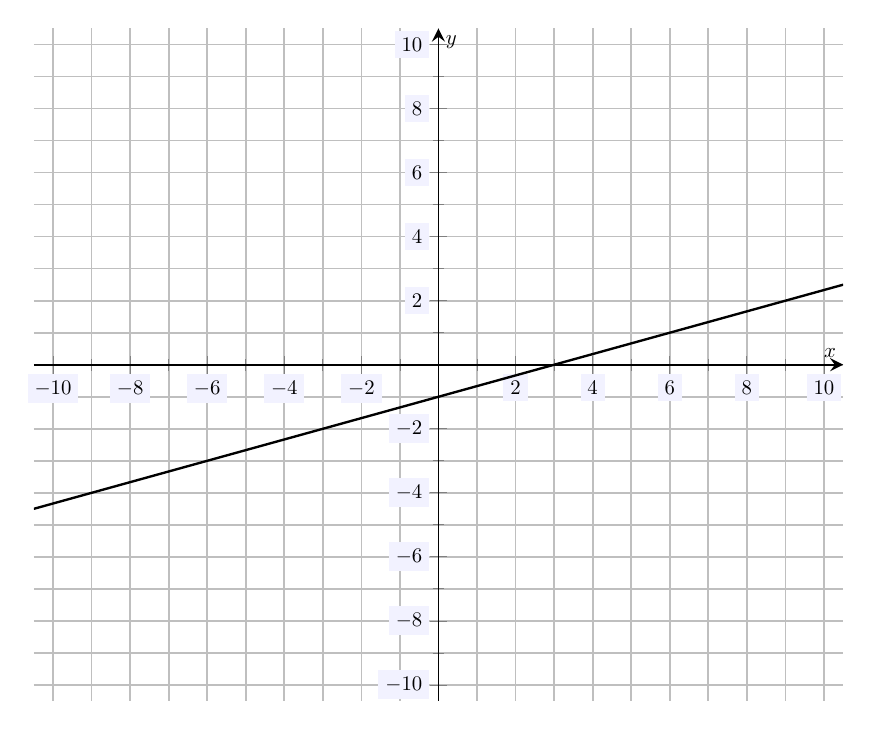
\begin{tikzpicture}[scale=1.5,every node/.style={scale=0.5}]
	\begin{axis}[
	grid=both,
	axis lines=middle,
	ticklabel style={fill=blue!5!white},
	xmin= -10.5, xmax=10.5,
	ymin= -10.5, ymax=10.5,
	xtick={-10,-8,-6,-4,-2,0,2,4,6,8,10},
	ytick={-10,-8,-6,-4,-2,0,2,4,6,8,10},
	minor tick = {-10,-9,...,10},
	xlabel=\(x\),ylabel=\(y\),
	]
	\addplot[line width= 0.02cm,samples=50,domain= -10.5:10.5] ({x},{1/3*x - 1});
	\end{axis}
	\end{tikzpicture}
	}
	\] 



% Question 6
\newpage
\question[10] Find the equation of the line with $x$-intercept $-6$ that passes through the point of intersection of $y= 5x - 1$ and $y= 6 - 2x$. 



% Question 7
\newpage
\question[10] Consider the lines $\ell_1(x)= 6x - 17$ and $\ell_2(x)= 8 - 11x$. 
	\begin{enumerate}[(a)]
	\item Determine whether the given lines are parallel, perpendicular, or neither. Justify your answer.
	\item Do the lines intersect? If not, explain why. If so, find their point of intersection. 
	\end{enumerate}



% Question 8
\newpage
\question[10] Consider the function given by $f(x)= 11 - 9x$.
	\begin{enumerate}[(a)]
	\item Explain why $f^{-1}(x)$ exists. 
	\item Find $f^{-1}(x)$.
	\item Use $f^{-1}$ to solve the equation $f(x)= \frac{17}{9}$. 
	\end{enumerate}



% Question 9
\newpage
\question[10] An \textit{arithmetic sequence} is a list of numbers where the difference between one number and the next is always the same. For instance, 2, 6, 10, 14, 18, \dots is an arithmetic sequence because the difference between sequential terms is always 4, while the sequence 1, 2, 3, 5, 7, 10, 13, \dots is \textit{not} an arithmetic sequence because the difference between sequential terms is not constant. Let $S$ be the sequence 34, 57, 80, 103, 127, \dots. 
	\begin{enumerate}[(a)]
	\item Find a function $S(n)$ that gives the $n$th term of the sequence. 
	\item Find the 835th term of the sequence. 
	\item Is 3,500 a term of this sequence? Explain. 
	\end{enumerate}



% Question 10
\newpage
\question[10] A cleaning service does not have their prices listed on their website but the site does mention they charge a fixed amount per hour. You make some calls and have one friend that used their service and paid \$212.50 for a 3~hour cleaning while another friend paid \$400 for a 6~hour cleaning. Let $C(h)$ be the cost the service will charge for $h$~hours of cleaning.
	\begin{enumerate}[(a)]
	\item Explain why $C(h)$ is linear.
	\item Find $C(h)$.
	\item Interpret the slope and $y$-intercept for $C(h)$.
	\item How many hours of cleaning can you get for \$950?
	\end{enumerate}


\end{questions}
\end{document}